% !TEX root = ./main.tex
\section{Status}
Until now we have been using a combination of Bash, Python and R. Preprocessing is done in Python, while the plots have been done in R. To run the preprocessing and then perform the plots, a few Bash scripts have been created. Tests have been performed using the labelled raw data. An example of a density plot has been included, see figure~\ref{fig:density}.

When finding the peak ID's, we used the euclidean distance for the distance measure. The first input file would become the baseline for the peaks. When reading some peak, we search in the baseline to find the peak that is closest to the new peak. If the closest peak is below the threshold it will get the same ID, if not then it would get a new peak ID. We plan to implement a method in the next few weeks that performs k-Means clustering on the data to find the peak ID's.

The indicator matrix is created by going through the output of finding the peak ID's and formatting it as an indicator matrix with samples on one dimension and peaks on the other dimension. The value at a given place of the indicator matrix would indicate whether the sample contains the peak or not.

At this point we are looking at using the package \texttt{randomForest} in R with the indicator matrix. After this, we will be looking at the package \texttt{cvTools} in R for cross-validation.
\newpage
\begin{figure}[h]
\centering
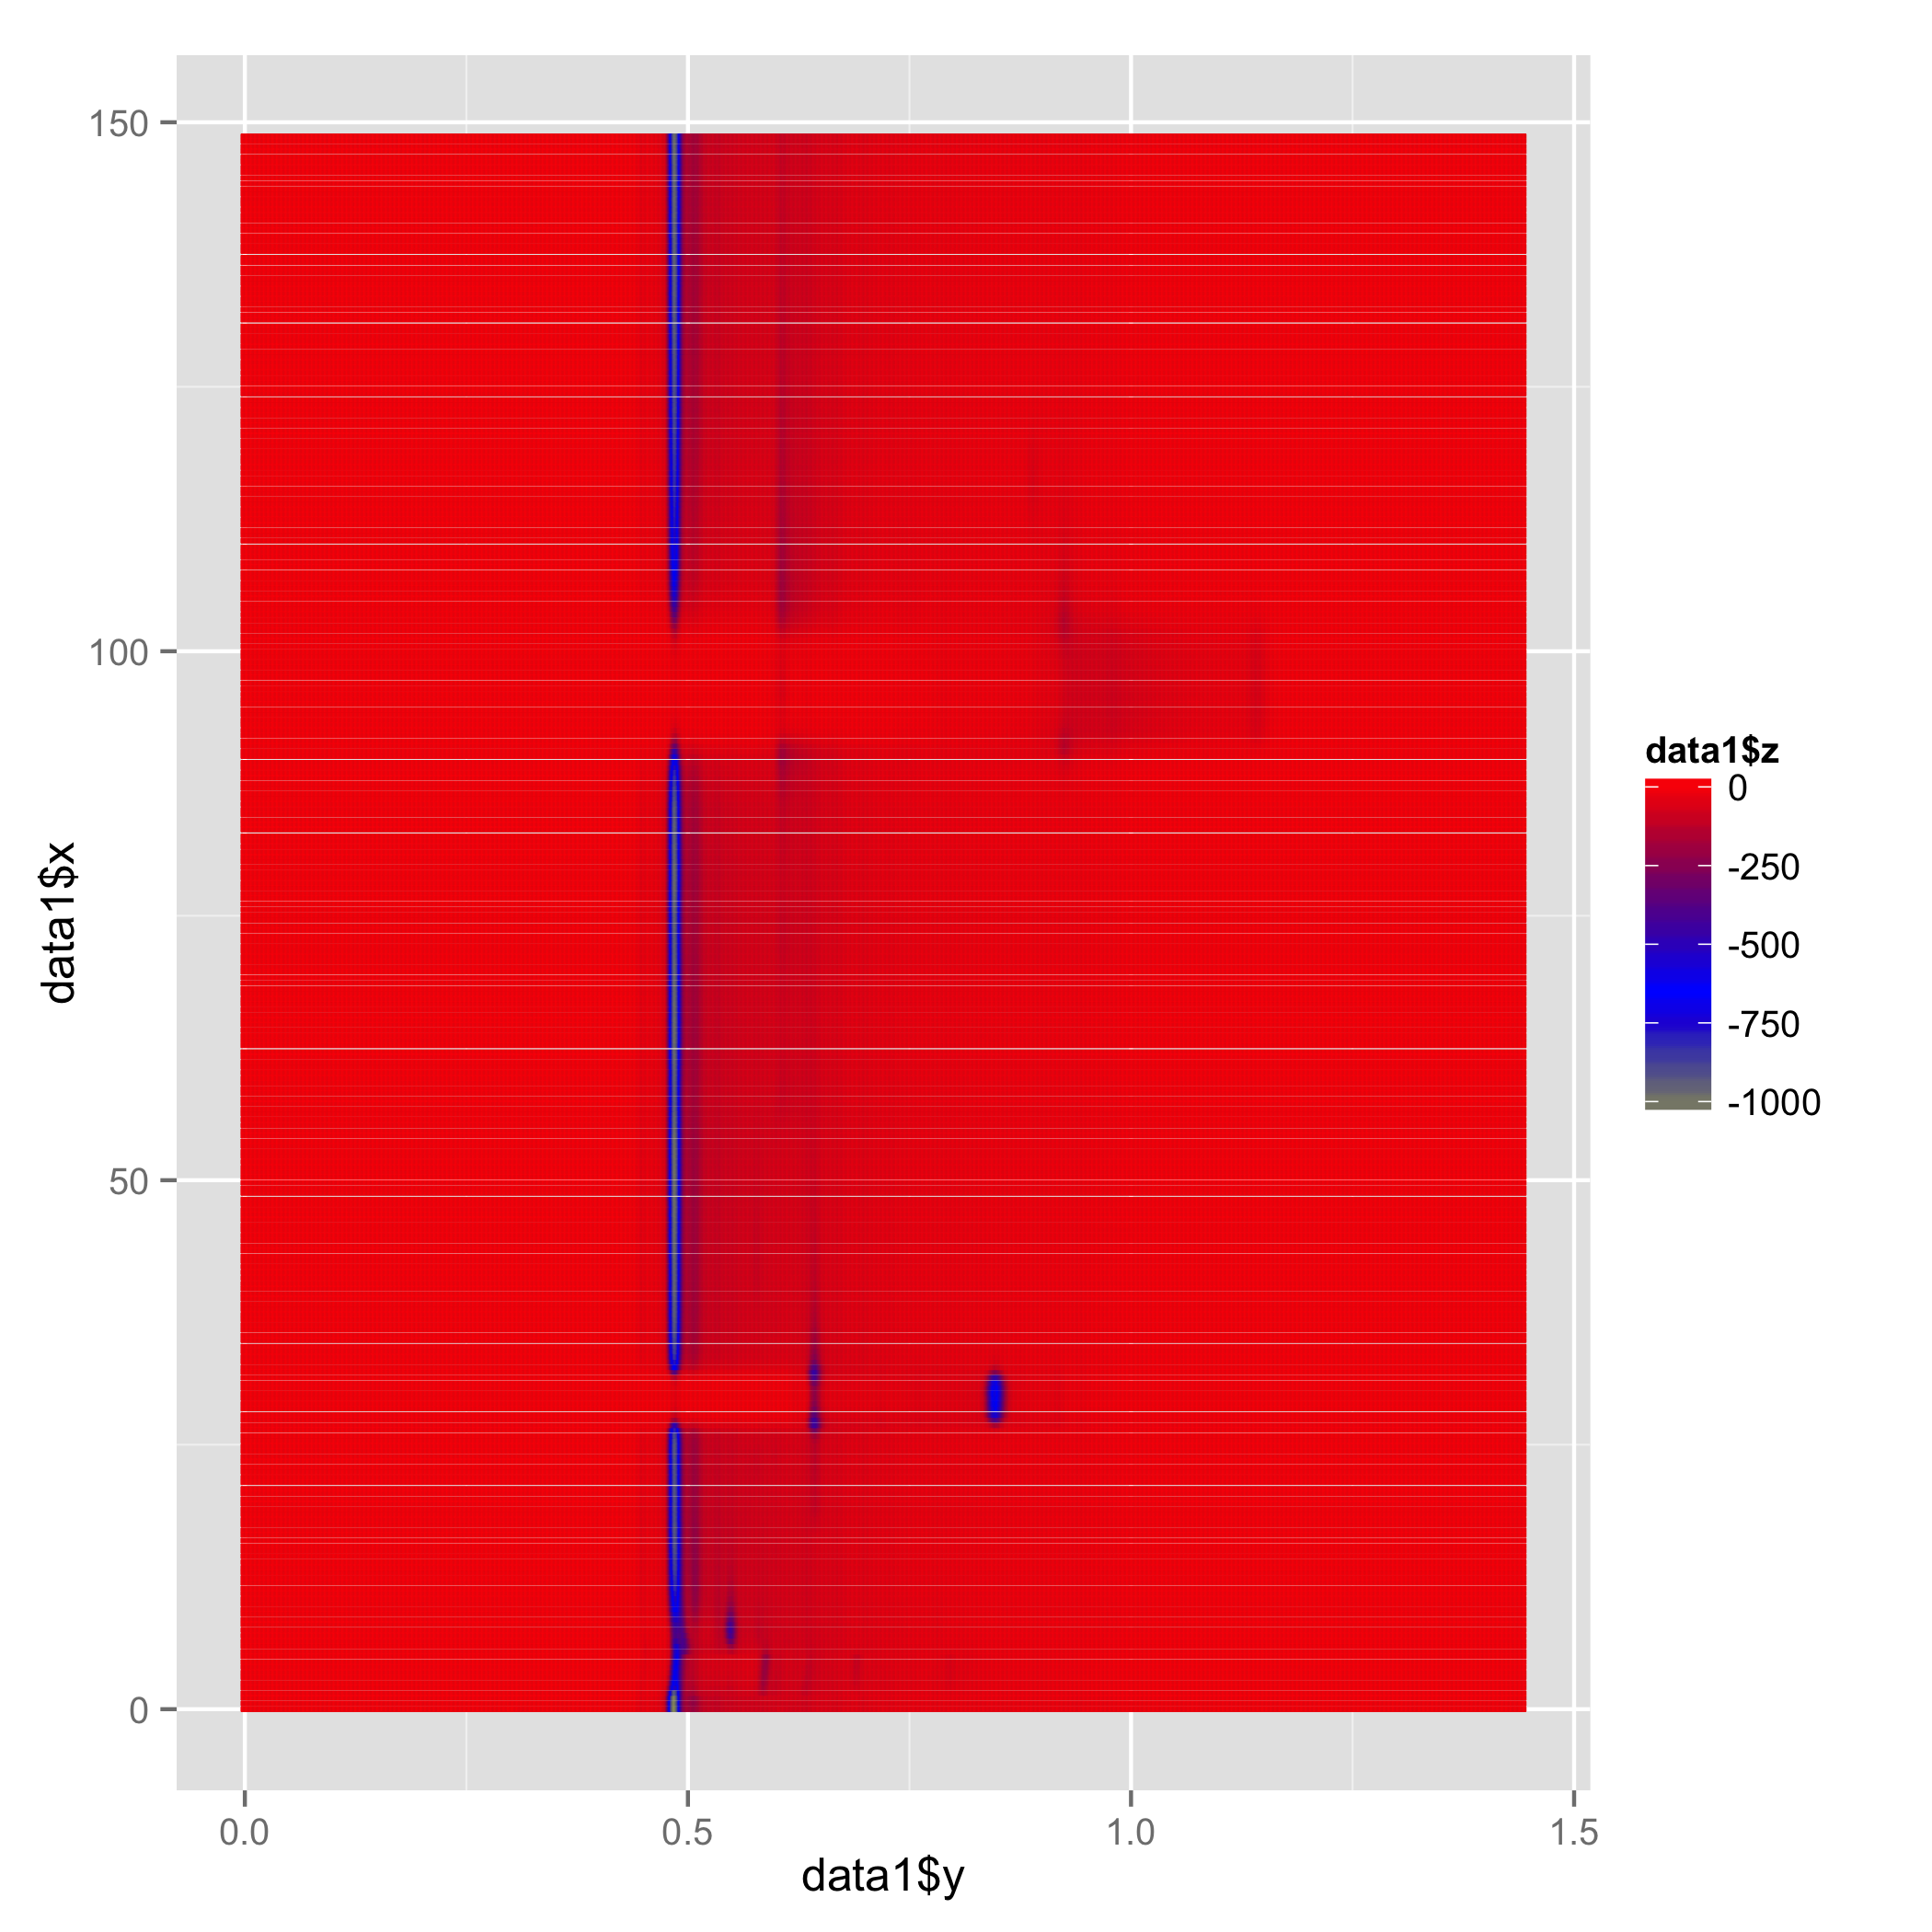
\includegraphics[width=1.00\textwidth]{../../plots/density/BD18_1411061750_ims.png}
\caption{Density plot for sample \texttt{BD18\_1411061750}.}
\label{fig:density}
\end{figure}

\begin{figure}[h]
\centering
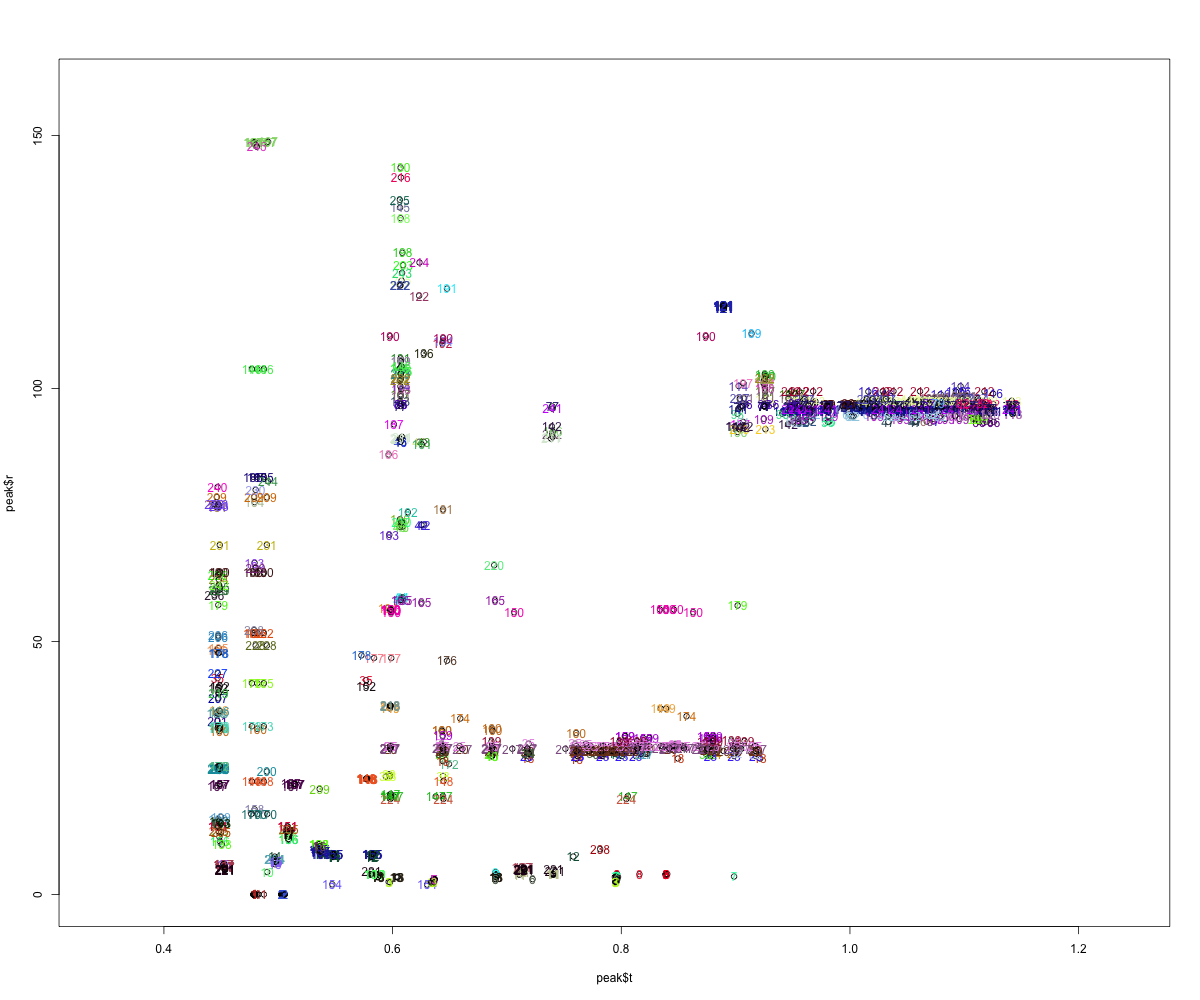
\includegraphics[width=1.00\textwidth]{../../plots/peak/peakoutput.png}
\caption{Peak alignment plot.}
\label{fig:peak_align}
\end{figure}

\begin{figure}[h]
\centering
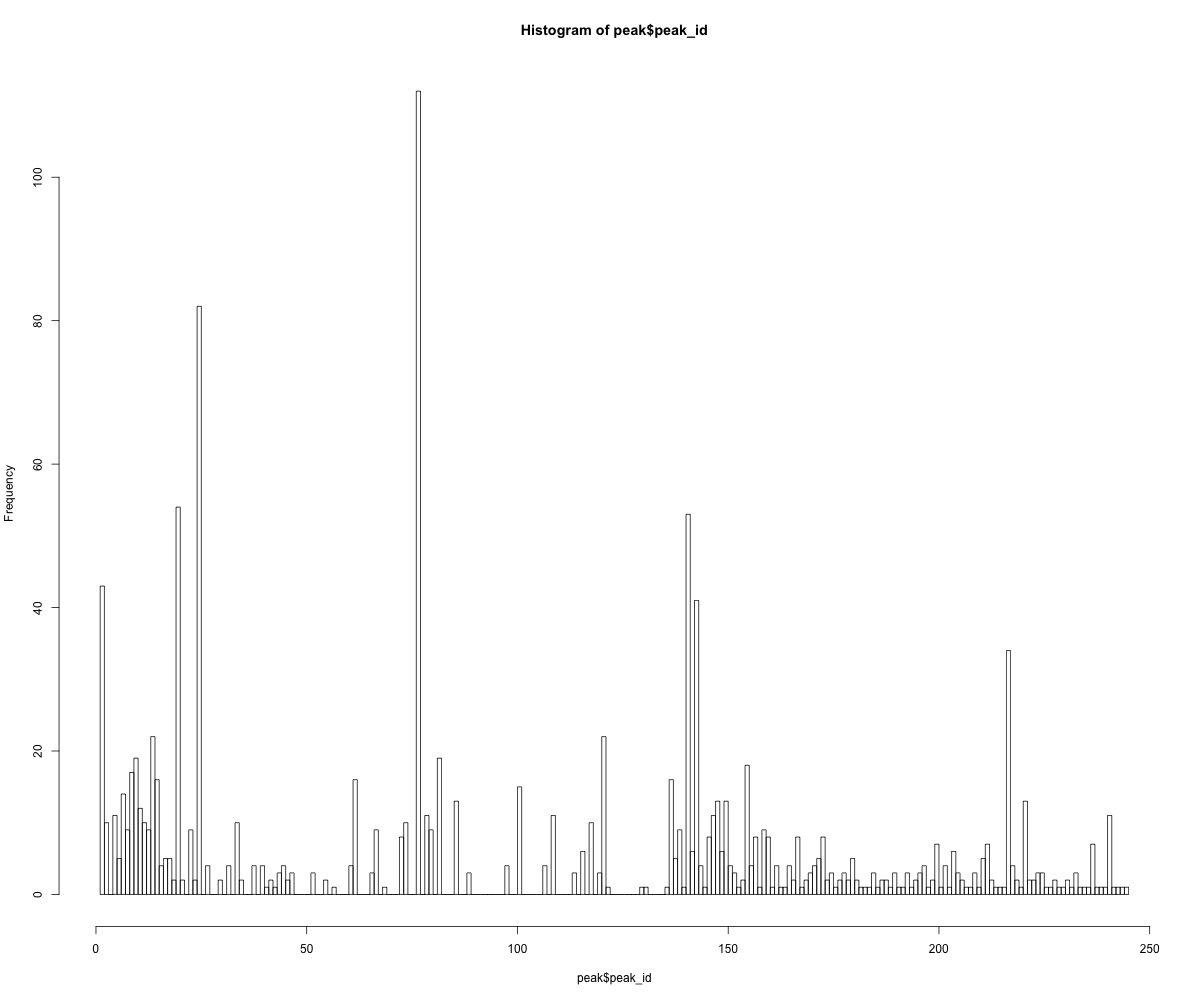
\includegraphics[width=1.00\textwidth]{../../plots/peak/peakoutput_histogram.png}
\caption{Histogram of peak ID's.}
\label{fig:peak_hist}
\end{figure}